\chapter*{Introduction}
\addcontentsline{toc}{chapter}{Introduction}

	To this day, turbulent motion of fluids remains the last unresolved problem of classical physics. They present many practical challenges across different areas of industry (e.g. weather prediction). Quantum turbulence, in contrast, may occur only in superfluids and was first observed in superfluid state of $\He$. Compared to classical turbulence, it can be regarded as a simpler system from the theoretical and numerical point of view. Also, it shares many of the general properties of turbulence in classical viscous fluids.

	In very low temperatures, the liquid state of $\He$ exists in two phases:
	\begin{itemize}
		\item \underline{Helium-I}: a high temperature liquid phase ($2.17\unit{K}<T<4.2\unit{K}$)
		\item \underline{Helium-II}: a low temperature superfluid phase ($T<2.17\unit{K}$)
	\end{itemize}

	These two phases are connected with the \textit{lambda transition}, as sketched in \textbf{Figure \ref{phase_diag}}, which occurs at the critical temperature $T_{\lambda} = 2.17 \unit{K}$ at saturated vapor pressure . Helium-I is a classical fluid described by ordinary Navier-Stokes (N-S) equations, whereas Helium-II is a superfluid and behaves partly like a Bose-Einstein condensate.

	\begin{figure}[h]
		\centering
		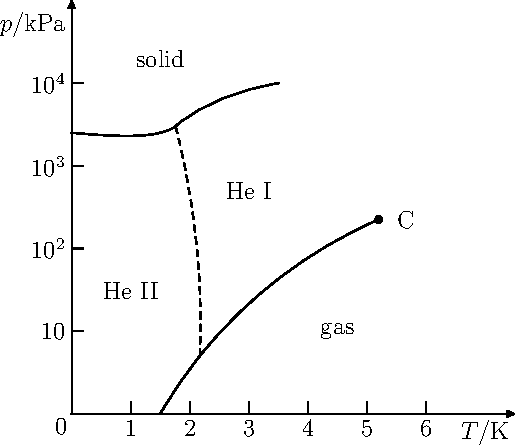
\includegraphics[width=0.6\textwidth]{graphics/theory/phase_diag}
		\caption{Pressure-Temperature diagram of $\He$. With a fixed pressure on the atmospheric value, a gas-liquid transition is present at temperature $4.2\unit{K}$ (He-I) and a superfluid transition near $2.17\unit{K}$.}
		\label{phase_diag}
	\end{figure}

	A simple, phenomenological model of the Helium-II composition was proposed by Tisza \cite{tisza} and Landau \cite{landau}, called as \textit{two-fluid model}. According to this model, Helium-II behaves as if composed of two inter-penetrating liquids - a \textit{normal} and a \textit{superfluid} component - with corresponding velocity fields and temperature-dependent, described as:

	\begin{itemize}
		\item \underline{normal component}: density $\rho_n (T)$, velocity field $\vec{v}_n (\vec{r}, t)$, motion described by an ordinary viscous Navier-Stokes equation, carrying entropy and represented as a collection of thermal excitations.
		\item \underline{superfluid component}: density $\rho_s (T)$, velocity field $\vec{v}_s(\vec{r}, t)$, motion described by a modified Euler equation (without viscosity) with quantum terms, carrying zero entropy and represented by a macroscopic wave function.
	\end{itemize}

	The total density of Helium-II sums up to $\rho = \rho_n(T) + \rho_s(T) \approx \text{const}$ and the relative proportion of normal/superfluid component is determined mainly by the temperature, as plotted in \textbf{Figure \ref{densities}}.\\
	Near $T \rightarrow 0$ Helium-II becomes entirely superfluid $\rho_s/\rho \rightarrow 1$, however, the temperature dependence of this ratio is highly nonlinear. For instance, the ratio $\rho_n/\rho$ drops from $100\%$ at $2.17\unit{K}$ to $50\%$ at $1.95\unit{K}$, to $<5\%$ at $1.3\unit{K}$, and is effectively negligible under $1\unit{K}$.

	\begin{figure}[h]
		\centering
		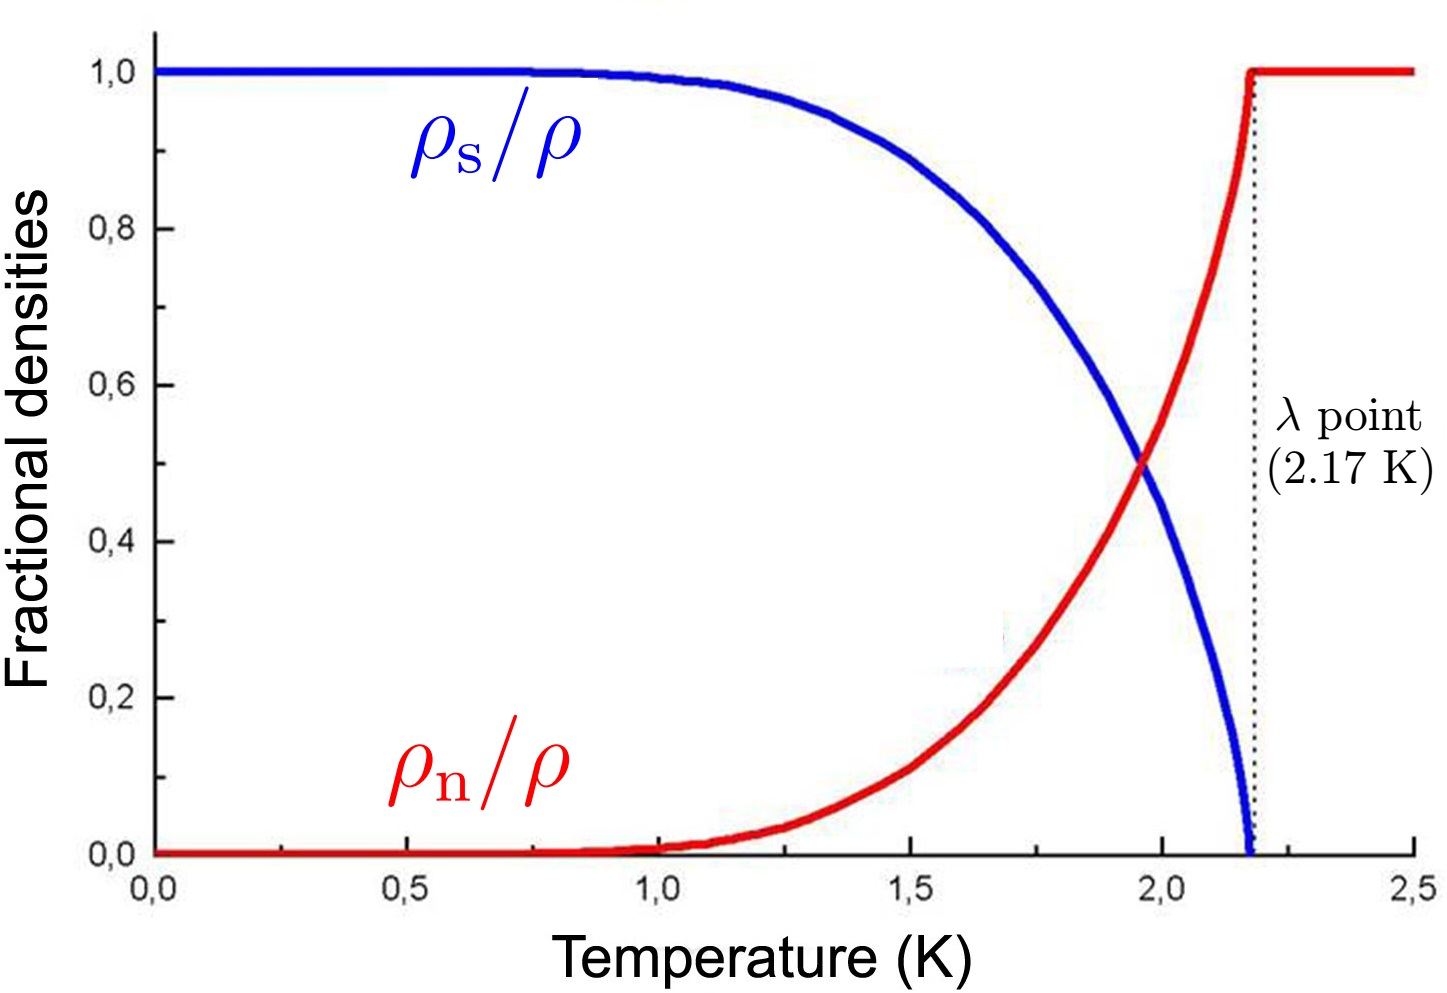
\includegraphics[width=0.6\textwidth]{graphics/theory/densities}
		\caption{Temperature dependence of fractional densities of the normal (red) and superfluid (blue) components. Source:\cite{svoc2016}}
		\label{densities}
	\end{figure}

	It arises from the quantum nature of Helium-II, that the superfluid component should not perform any rotation. However, when this component moves faster than a critical velocity, the circulation is \textit{quantized} and so-called \textit{quantized vortices} are created, which makes the hydrodynamics of Helium-II particularly interesting. However, the vortex nucleation process is still a subject of many current investigations.\\
	Superfluid vortex lines were observed spatially organized \cite{bewley}, but also completely disorganized as showed also by a simulation in \textbf{Figure \ref{sim_cube}}. Quantum turbulence therefore usually takes the form of a chaotic tangle of quantized vortices in the superfluid component which typically coexist with classical turbulent flow of the normal component.

	In the presence of quantized vortices, the seemingly independent normal and superfluid velocity fields become coupled by the \textit{mutual friction} force which arises due to quasiparticles scattering off the cores of vortices. More details about this interaction are provided in \textbf{Theoretical Background} chapter.

	\begin{figure}[h]
		\centering
		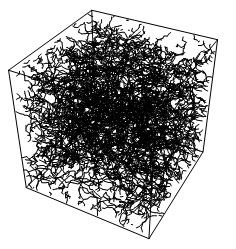
\includegraphics[width=0.35\textwidth]{graphics/theory/QT-tangle}
		\caption{Cube of numerically simulated tangle of randomly distributed quantized vortices. Source:\cite{svoc2016}}
		\label{sim_cube}
	\end{figure}

	Quantum turbulence can be experimentally achieved in many traditional ways - driving a mass flow, spinning discs, oscillating grids and forks, ultrasound and jets. In order to characterize the turbulence, one may use a superfluid Reynolds number for steady flows, or a newly introduced (the last section of \textbf{Theoretical Background} chapter) \textit{Donnelly number} for high-frequency oscillatory flows.\\
	We find (see \textbf{Results} chapter) that for quantum turbulence originated in such high-frequency oscillation regime at temperatures $T > 1\unit{K}$, the measured drag forces are described in terms of a single dimensionless parameter and exhibit an \textit{universal scaling} behavior. We identify and compare the critical conditions related to the production of both quantized vorticity and instabilities occurring in normal component.

	Also we note that if we cool the experimental system below $\lesssim 0.6\unit{K}$, a transition to ballistic regime occurs in the normal component, as the mean free path of phonons exceeds the characteristic dimensions of the experimental setup. This situation is similar to the one of dilute classical gases, so the hydrodynamical description of the system is no longer valid. We discuss the applicability of \textit{universal scaling} for such system in \textbf{Conclusions} chapter.

	Besides experimental approaches on quantum fluids, one of the useful tools for understanding the geometry and flow of quantum turbulence, is the \textit{vortex filament model}, pioneered by Schwarz \cite{schwarz} in late 80's. With the rapid development of available computational power, large simulations have become the methods of choice for calculating the motion of fluids. In superfluids like Helium-II, due to the quantization of circulation, vorticity can only exist within vortex filaments with a certain core size, which makes the model highly applicable.

	In this Thesis, we also propose an efficient numerical method to compute the time evolution of vortex filaments in superfluid Helium-II. We studied the performance and stability and well replicated the physical processes such as the annihilation of quantized vortex rings \cite{vortex_ring} phenomena while traveling across superfluid.\\
	Hence, we present the \texttt{PyVort} codebase, a new platform in \texttt{Python 3} to simulate quantized rings motion. The implementation details are provided in \textbf{Simulation} chapter.

%%%%%%%%%%%%%%%%%%%%%%%%%%%%%%%%%%%%%%%%%%%%%%%%%%%%%%%%%%%%%%%%%%%%%%%%%%%%%%

	\section*{Motivations and Goals}
	\addcontentsline{toc}{chapter}{Motivations and Goals}

	Here we briefly present all motivations and goals plan that led us to our investigations with oscillators in superfluid Helium-II and vortex simulations we performed.

	\subsection*{Experiments and Data analysis}

	\begin{itemize}
		\item \textbf{construct} a low-temperature experiment using flow generators such as \textit{vibrating wire, tuning fork and oscillating disc} in order to observe the drag phenomena
		\item \textbf{investigate} transition from laminar/potential flow of normal/superfluid components, respectively, to \textit{classical, quantum and mixed turbulence} at various temperatures $T > 1\unit{K}$ in a high-frequency regime.
		\item \textbf{apply} universal scaling method, \textbf{prove} the concept on collected experimental data and \textbf{test} the limitations using the ultra-low temperature data
	\end{itemize}

	\subsection*{Simulation}
	\begin{itemize}
		\item \textbf{build} modular and reusable codebase in \texttt{Python 3} that simulates the dynamics of quantized vortices using the \textit{Vortex Filament} model
		\item \textbf{implement} stable \textit{stepping methods} and a reliable \textit{re-segmentation process} that allows keeping a good resolution of quantized vortices in different situations
		\item \textbf{simulate} a real-time vortex ring motion and \textbf{compare} its properties evolving in time with the theoretical approaches, thus \textbf{validating} the new codebase
	\end{itemize}

\newpage

%%%%%%%%%%%%%%%%%%%%%%%%%%%%%%%%%%%%%%%%%%%%%%%%%%%%%%%%%%%%%%%%%%%%%%%%%%%%%%
%%%%%%%%%%%%%%%%%%%%%%%%%%%%%%%%%%%%%%%%%%%%%%%%%%%%%%%%%%%%%%%%%%%%%%%%%%%%%%
%%%%%%%%%%%%%%%%%%%%%%%%%%%%%%%%%%%%%%%%%%%%%%%%%%%%%%%%%%%%%%%%%%%%%%%%%%%%%%

\chapter{Theoretical Background}

The theoretical part of this Thesis is composed of two chapters:

\begin{itemize}
	\item[1.] \underline{Micro/Meso-scopic view} - provides a theoretical cover of Gross-Pitaevskii model of Helium-II, quantized vortex description, properties and motion, numerical modeling of such vortex and a brief view on quantized ring dynamics

	\item[3.] \underline{Macroscopic view} - provides a hydrodynamic description of two-fluid model, dynamical similarity principle, oscillatory flows in both classical viscous and superfluid He-II, creation of quantum turbulence, universal scaling principles and ultra-low temperature regime differences

\end{itemize}

The aim of this chapter is to introduce the basic properties of quantized vortex lines in Helium-II and summarize the state of art of current knowledge on superfluid turbulence. We also discuss the theoretical methods used to study quantized vorticity, quantum turbulence and some results obtained using such methods.

%%%%%%%%%%%%%%%%%%%%%%%%%%%%%%%%%%%%%%%%%%%%%%%%%%%%%%%%%%%%%%%%%%%%%%%%%%%%%%
%%%%%%%%%%%%%%%%%%%%%%%%%%%%%%%%%%%%%%%%%%%%%%%%%%%%%%%%%%%%%%%%%%%%%%%%%%%%%%

\newpage

{\Huge \bfseries Micro/Meso-scopic view}
\addcontentsline{toc}{chapter}{Micro/Meso-scopic model}
\vspace{0.3cm}

One of the most useful ways of describing superfluid $\He$ at $T=0\unit{K}$ starts with nonlinear Schrodinger equation (NLSE) for the one-particle wave function $\psi$. Since the superfluid $\He$ is a strongly correlated system dominated by collective effects, this imperfect Bose-Einstein condensate (BEC) is approximately described by Gross-Pitaevskii equation (\ref{gross-pit}). Although, it must be noted that the real Helium-II is a dense fluid, not a weakly interacting Bose gas described by NLSE.

%%%%%%%%%%%%%%%%%%%%%%%%%%%%%%%%%%%%%%%%%%%%%%%%%%%%%%%%%%%%%%%%%%%%%%%%%%%%%%

\section{Gross-Pitaevskii model}

In terms of single-particle wavefunction $\psi(\vec{r},t)$ we write the Gross-Pitaevskii model:

\begin{equation}
i \hbar \frac{\partial \psi}{\partial t} = - \frac{\hbar^2}{2m} \nabla^2 \psi
+ \psi \int \vert \psi(\vec{r}^{\prime},t) \vert^2 V(\vert \vec{r} - \vec{r}^{\prime} \vert)
\text{d}\vec{r}^{\prime}\,,
\label{gross-pit}
\end{equation}

where $V(\vert \vec{r} - \vec{r}^{\prime} \vert)$ is the potential of two-body interaction between bosons. The normalization is set as $\int \vert \psi \vert^2 \text{d}\vec{r} = N$, where $N$ is number of bosons. By replacing potential with repulsive $\delta$-function of strength $V_0$ one obtains:

\begin{equation}
i \hbar \frac{\partial \Psi}{\partial t} = - \frac{\hbar^2}{2m} \nabla^2 \Psi - m\eps \Psi + V_0 \vert \Psi \vert^2 \Psi\,,
\label{GP}
\end{equation}

where $\eps$ is the energy per unit mass and $\Psi = A e^{i\Phi}$ is a macroscopic wave function of condensate. In this way one can define the condensate's density $\rho_{BEC} = m\Psi\Psi^* =  mA^2$ and velocity $\vec{v}_{BEC} = (\hbar / m)\nabla \Psi$. Note that equation (\ref{GP}) is equivalent to a continuity equation and a Euler equation (however, modified by the so called \textit{quantum pressure term}).

Hereafter we identify $\rho_{BEC}$ with $\He$ superfluid component's $\rho_s$ at absolute zero and $\vec{v}_{BEC}$ with $\vec{v}_s$. It must be noted that this identification is convenient from the point of view of having a simple hydrodynamics model but is not entirely correct. The reason is
that Helium-II is a dense fluid, not the weakly interacting Bose gas described
by the NLSE (\ref{gross-pit}), so the condensate is not the same as the superfluid component.

\newpage

Even though the superfluid is irrotational: $\omega = \nabla \times \vec{v}_s = \vec{0}$, the NLSE has a vortex-like solution: $\vec{v}_s = \varkappa / 2\pi r\, \vec{e_{\theta}}$, where $\theta$ is the azimuthal angle and $\varkappa=9.97 \times 10^{-8} \unit{m^2/s}$ is the \textit{quantum of circulation}, obtained from:

\begin{equation}
\varkappa = \oint_{\mathcal{C}} \vec{v}_{BEC} \cdot \unit{d}\vec{\boldsymbol{\ell}} = \frac{h}{m}\,,
\label{varkappa}
\end{equation}

where $\mathcal{C}$ is a closed loop surrounding the vortex core - a topological defect within macroscopic wavefunction $\Psi$, as sketched in \textbf{Figure \ref{singularity}}.

\begin{figure}[h]
	\centering
	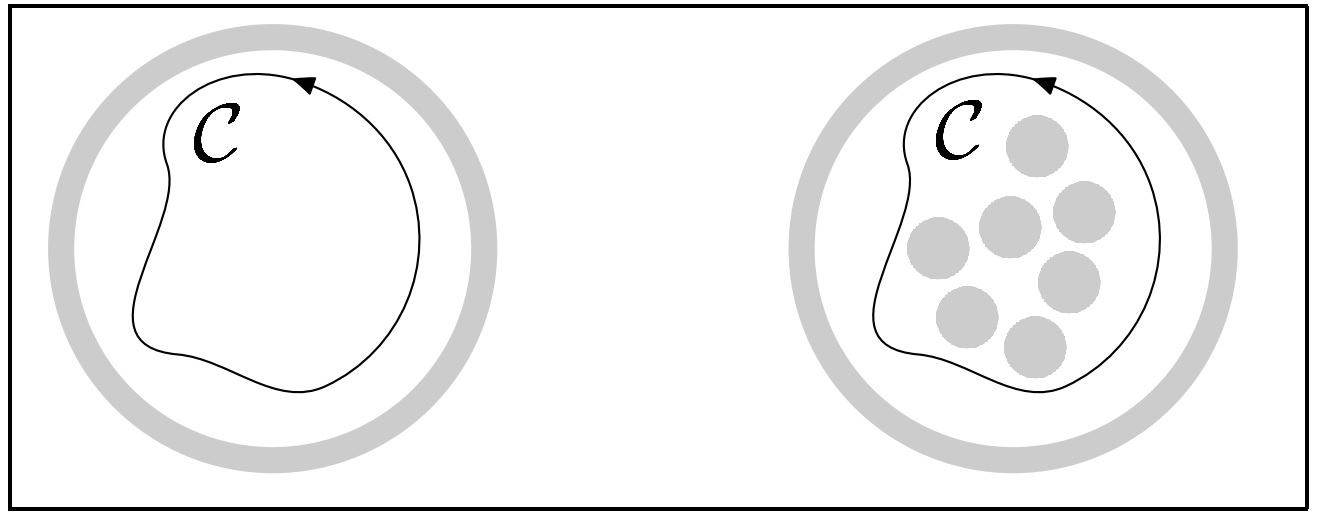
\includegraphics[width=0.6\textwidth]{graphics/theory/singularity}
	\caption{An illustration of topological singularities within a superfluid $\He$. Left: A singly-connected irrotational region with circulation along $\mathcal{C}$ loop equal to zero. Right: A multiply-connected region with depicted cores of quantized vortices with a finite circulation along $\mathcal{C}$ loop.}
	\label{singularity}
\end{figure}

%%%%%%%%%%%%%%%%%%%%%%%%%%%%%%%%%%%%%%%%%%%%%%%%%%%%%%%%%%%%%%%%%%%%%%%%%%%%%%

\section{Quantized vortex}

As Feynman showed \cite{feynman}, superfluid vortex lines appear when Helium-II moves faster than a certain critical velocity. The simplest way to create quantized vortices is to rotate cylinder with superfluid Helium-II with high enough angular velocity $\Omega$. Created vortex lines form an ordered array of density $L=2\Omega / \varkappa$, all aligned along the axis of rotation, as sketched in \textbf{Figure \ref{rotating-helium}}. \textit{Vortex line density} $L$ is usually interpreted as a total vortex length in an unit volume.

The key properties of Onsager-Feynman vortex \cite{onsager} are the quantized circulation $\varkappa$, local superfluid rotational velocity field $v_s = \varkappa / 2\pi r$ and the \textit{vortex core size} $a_0$. The core size $a_0$ can be estimated by substituting $v_s$ back into equation (\ref{GP}) and solving the resultant differential equation for $\rho_s (\vec{r})$. One finds that $\rho_s (\vec{r})$ tends to the bulk value $m^2 \eps / V_0$ for $r \rightarrow \infty$ from the vortex and to zero density for $r \rightarrow 0$.
The characteristic distance over which $\Psi$ collapses (superfluid density $\rho_s$ drops $m^2 \eps / V_0 \rightarrow 0$) is $a_0 \approx 10^{-10} \unit{m} \equiv 1 \unit{\AA}$. From this, there is a conclusion that the vortex is hollow at its core and therefore, a topological defect occurs.

Taking $a_0$ as core radius, the energy considerations showed that a single vortex containing $N$ circulation quanta owns more energy than $N$ singly-quantized vortices. Hence it is generally assumed that only ground-state vortices are commonly observed.

\begin{figure}[h]
	\centering
	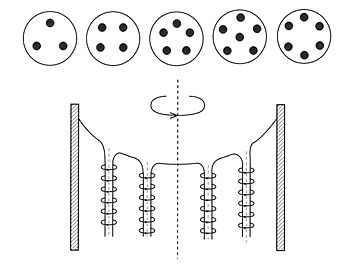
\includegraphics[width=0.4\textwidth]{graphics/theory/rotating-helium}
	\caption{Array of quantized vortices in a rotating container. The 5 images at the top mark the position of various number of vortex lines from the upper point of view.}
	\label{rotating-helium}
\end{figure}

Clearly, vortex lines don't have to be aligned in general. In most cases , the superfluid flow is strongly chaotic, better known as \textit{quantum turbulence}. This topic is covered in more detail later in this work.

%%%%%%%%%%%%%%%%%%%%%%%%%%%%%%%%%%%%%%%%%%%%%%%%%%%%%%%%%%%%%%%%%%%%%%%%%%%%%%

\section{Vortex filament model}

The vortex line can be represented as a curve via position vector $\vec{s} = \vec{s}(\xi, t)$ in three-dimensional space. Here, $\xi$ is arclength along the vortex line. Next we label $\vec{s}^{\prime}$ as $\text{d}\vec{s} / \text{d} \xi$ and $\vec{s}^{\prime\prime}$ as $\text{d}\vec{s}^{\prime} / \text{d} \xi$.
Within our context, $\vec{s}^{\prime}$ is a tangent vector and $\vert \vec{s}^{\prime\prime} \vert$ is a local curvature $R^{-1}$ at a given point.
The triad of vectors $\vec{s}^{\prime}$, $\vec{s}^{\prime\prime}$, $\vec{s}^{\prime} \times \vec{s}^{\prime\prime}$ are perpendicular to each other, as sketched in \textbf{Figure \ref{filament}}, and point along the tangent, normal and binormal respectively:

\begin{figure}[h]
	\centering
	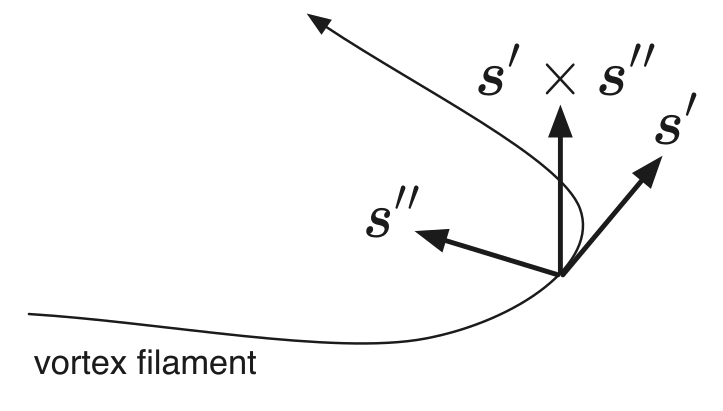
\includegraphics[width=0.6\textwidth]{graphics/theory/filament}
	\caption{Schematic of the vortex filament and the triad vectors $\vec{s}^{\prime}$, $\vec{s}^{\prime\prime}$, $\vec{s}^{\prime} \times \vec{s}^{\prime\prime}$. Source:\cite{tsubota}}
	\label{filament}
\end{figure}

We suppose that the superfluid component is incompressible $\nabla \dotprod \vec{v}_s = 0$. Moreover, superfluid vorticity $\omega_s$ is localized only at positions of vortex filament $\omega_s(\vec{r},t) = \nabla \times \vec{v}_s$. Combining these two properties gives the Poisson equation $\Delta \phi = \omega_s$ for the potential $\phi$.
Using Fourier transform one obtains \cite{barenghi} the Biot-Savart law for the superfluid velocity:

\begin{equation}
\vec{v}_s(\vec{r}) = \frac{\varkappa}{4\pi} \int_{\mathcal{L}} \frac{(\vec{r^{\prime}} - \vec{r}) \times \text{d}\vec{r^{\prime}}}{\vert \vec{r^{\prime}} - \vec{r} \vert^3}\,,
\label{biot_general}
\end{equation}

where the integral path $\mathcal{L}$ represents curves along all vortex filaments.

This law determines the superfluid velocity field $\vec{v}_s(\vec{r})$ via the arrangement of the vortex filaments. Now we define the \textit{self-induced} velocity $\vec{v}_{\text{ind}}$, describing the motion which a vortex line induces onto itself ($\vec{r} \rightarrow \vec{s}$ in (\ref{biot_general})) due to its own curvatures:

\begin{equation}
\vec{v}_{\text{ind}}(\vec{s}) = \frac{\varkappa}{4\pi} \int_{\mathcal{L}} \frac{(\vec{r^{\prime}} - \vec{s}) \times \text{d}\vec{r^{\prime}}}{\vert \vec{r^{\prime}} - \vec{s} \vert^3}
\label{biot_ind}
\end{equation}

However, this integral (\ref{biot_ind}) diverges as $\vec{r}^{\prime} \rightarrow \vec{s}$ because the core structure
of the quantized vortex was initially neglected. We avoid this divergence by splitting the integral into two parts - direct neighborhood of the point $\vec{s}$ (local part) and the rest $\mathcal{L}^{\prime}$ (nonlocal part). The Taylor expansion of the local part leads \cite{schwarz} to a finite result:

\begin{align}
\vec{v}_{\text{ind}}(\vec{s})
= \vec{v}_{\text{ind,local}} + \vec{v}_{\text{ind,nonlocal}}
\approx& \beta \vec{s}^{\prime} \times \vec{s}^{\prime \prime} + \frac{\varkappa}{4\pi} \int_{\mathcal{L}^{\prime}} \frac{(\vec{r^{\prime}} - \vec{s}) \times \text{d}\vec{r^{\prime}}}{\vert \vec{r^{\prime}} - \vec{s} \vert^3}\,,
\label{lia+biot}
\\
\text{where}\, \beta =& \frac{\varkappa}{4\pi} \ln(R / a_0)\,,
\label{beta}
\end{align}

where $\mathcal{L}^{\prime}$ is the original vortex line without a close area of the studied vortex point and $R$ is a \textit{local curvature} and often is calculated as $1 / \vert \vec{s}^{\prime\prime} \vert$ \cite{schwarz}.

Since the local part of induced velocity (\ref{lia+biot}) is a dominant term (and also computationally faster), the nonlocal part can be neglected. Such approximation process is called as \textit{Local Induction Approximation} (LIA). LIA represents the contribution of local curvature to the induced velocity, whereas nonlocal Biot-Savart part represents the global filament curvature.

Since in the system there could be present also external flow sources of superfluid component (e.g. heat resistors causing \textit{counterflows}), we define the total superfluid velocity $\vec{v}_{s,tot}$, in a laboratory frame, as:

\begin{equation}
\vec{v}_{s,tot} = \vec{v}_{s,ext} + \vec{v}_{\text{ind}}
\end{equation}

\newpage

%%%%%%%%%%%%%%%%%%%%%%%%%%%%%%%%%%%%%%%%%%%%%%%%%%%%%%%%%%%%%%%%%%%%%%%%%%%%%%


\section{Vortex dynamics}

To determine the equation of motion of $\vec{s}(t)$ we recognize the forces acting upon the line - the Magnus force $\vec{f}_M$ and (at non-zero temperature $T>0\unit{K}$ )the drag force $\vec{f}_D$ (both are per unit length).

The Magnus force $\vec{f}_M$ always arises when a rotating body moves in a flow. This causes a pressure difference, which in our case of moving vortex line with circulation quantum $\varkappa$, exerts a force:

\begin{equation}
\vec{f}_M = \rho_s \varkappa \,\vec{s}^{\prime} \times (\vec{\dot{s}} - \vec{v}_{s,tot})\,,
\label{magnus}
\end{equation}

where $\vec{\dot{s}} = \text{d}\vec{s} / \text{d} t$ is the velocity of a particular point on a vortex line.

The drag force $\vec{f}_D$ arises from the \textit{mutual friction}, the interaction between the normal component and vortex lines (quantized superfluid component). According to the findings of Vinen and Hall \cite{vinen}, the normal fluid flowing with velocity $\vec{v}_n$ past a vortex core exerts a frictional force $\vec{f}_D$ on the vortex line, given by:

\begin{align}
\vec{f}_D = -& \alpha(T)\rho_s\varkappa\,\vec{s}^{\prime} \times [\vec{s}^{\prime} \times (\vec{v}_{ns} - \vec{v}_{\text{ind}})]
\label{alpha1}
\\
-& \alpha^{\prime}(T)\rho_s\varkappa\,\vec{s}^{\prime} \times (\vec{v}_{ns} - \vec{v}_{\text{ind}})
\,,
\label{alpha2}
\end{align}

where $\vec{v}_{ns} = \vec{v}_{n} - \vec{v}_{s,ext}$ is the difference between the average velocity of normal component and the applied superfluid velocity.

The temperature dependent dimensionless parameters $\alpha(T)$ and $\alpha^{\prime}(T)$ are often written in terms of measured \textit{mutual friction parameters} $B$ and $B^{\prime}$, which are known from experiments by Samuels and Donnelly \cite{donnelly}:

\begin{equation}
\alpha(T) = \frac{\rho_n B(T)}{2\rho}
\hspace{1cm}
\alpha^{\prime}(T) = \frac{\rho_n B^{\prime}(T)}{2\rho}
\end{equation}

The precise calculation of the mutual friction parameters $B(T), B^{\prime}(T)$ over the entire temperature range is still an open problem. Although, we already know that in the area of high temperatures, the friction arises mainly from the scattering processes of rotons.

\newpage

Since the mass of vortex core is usually neglected, the two forces $\vec{f}_M$ and $\vec{f}_D$ add up to zero: $\vec{f}_M + \vec{f}_D = \vec{0}$. Hence, solving for $\text{d}\vec{s} / \text{d} t$, we obtain \cite{schwarz} the Schwarz's equation:

\begin{align}
\dot{s} =& \,\vec{v}_{\text{s, ext}} + \vec{v}_{\text{ind}} + \vec{v}_{\text{drive}}
\,,\,\, \text{where}
\label{schwarz}
\\
\vec{v}_{\text{drive}} =& \,\alpha\vec{s}^{\prime} \times (\vec{v}_{ns} - \vec{v}_{\text{ind}})
- \alpha^{\prime}\vec{s}^{\prime} \times [\vec{s}^{\prime} \times (\vec{v}_{ns} - \vec{v}_{\text{ind}})]
\label{drive}
\end{align}

On the basis of Schwarz's equation (\ref{schwarz}), algorithms to numerically simulate vortex time evolution of an arbitrary configuration can be developed. Also, the vortex parametrization $\vec{s}(\xi, t)$ and dynamics description provide the baseline of what we call as Vortex Filament (VF) model. More on VF model is written later in \textbf{Simulation} chapter.

%%%%%%%%%%%%%%%%%%%%%%%%%%%%%%%%%%%%%%%%%%%%%%%%%%%%%%%%%%%%%%%%%%%%%%%%%%%%%%


\subsection*{Quantized vortex rings}

A special case of vortex line configuration are a freely moving vortex rings. Such rings are usually created as a result of multi-vortex interconnections \cite{vortex_ring} or by the self-reconnection of an oscillating loop pinned to the surface of a vibrating body. The exact expressions derived from the Gross-Pitaevskii equation (\ref{gross-pit}) \cite{roberts} for the energy $E$ and induced center velocity $v_{\text{ind}}$ of a vortex ring, moving in a Helium-II of density $\rho$ and having a radius $R$ much greater than its core radius $R >> a_0$, are:

\begin{equation}
E = \frac{1}{2}\varkappa^2 \rho R \Big(\ln(8R/a_0) - 2 + c\Big)
\label{ring-energy}
\end{equation}

\begin{equation}
v_{\text{ind}} = \frac{\varkappa}{4\pi R} \Big(\ln(8R/a_0) - 1 + c\Big)\,,
\label{ring-velocity}
\end{equation}

where $c$ is a constant based on inner structure of the vortex. Since we work with hollow core, we use \cite{donnelly_book}
$c = 1/2$. Note that (\ref{ring-energy}) and (\ref{ring-velocity}) depend on $a_0$ only logarithmically.
The behavior of the vortex ring is thus quite insensitive to the exact value of $a_0$ (expected to be of the order of atomic dimension).

Relations (\ref{ring-energy}) and (\ref{ring-velocity}) are derived directly from Gross-Pitaevskii description and no dissipative process (mutual friction) was included. Therefore, the relations hold only for temperature $T=0\unit{K}$.\\
Using the explicit dynamical equation \cite{donnelly_book} for vortex ring motion, one can also derive the final ring center velocity $\vec{v}_{\text{ring}}$ and energy $E_{\text{ring}}$ using (\ref{ring-energy}) and (\ref{ring-velocity}) like:

\begin{equation}
\vec{v}_{\text{ring}} = (1 - \alpha^{\prime}) (\vec{v}_{\text{ind}} - \vec{v}_{\text{s, ext}})
+ \alpha^{\prime} \vec{v}_{\text{n, ext}}
\label{v_ring}
\end{equation}

\begin{equation}
E_{\text{ring}} = \Big( \frac{\alpha}{1 - \alpha^{\prime}} \Big) E
\label{E_ring}
\end{equation}

Several other interesting results come from the ring's dynamic motion equation and the mutual friction formula (\ref{alpha1}), (\ref{alpha2}). The second term (\ref{alpha2}) of friction force causes the decrease of vortex ring radius, whereas the first term (\ref{alpha1}) is the dissipative term. The superfluid vortex ring (\textbf{Figure (\ref{vortex-ring})}) living in a mixture of a normal and superfluid component has therefore a limited lifetime expectancy and the traveled distance.

\begin{figure}[h]
	\centering
	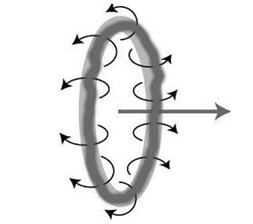
\includegraphics[width=0.4\textwidth]{graphics/theory/vortex-ring}
	\caption{Depiction of quantized vortex ring motion and induced velocity field. Source: Huang, Kerson, \textit{Quantum vorticity in nature}, arXiv.}
	\label{vortex-ring}
\end{figure}

More explicitly, it was shown \cite{donnelly_book} that in case of weak counterflow velocity $\vec{v}_{\text{ns}}$, the lifetime of vortex ring can be expressed as a simple relation:

\begin{equation}
\tau_{\text{ring}} = \frac{R_0}{2 \alpha \vert \vec{v}_{\text{ring}}(R_0)\vert}\,,
\label{ring-lifetime}
\end{equation}

where $R_0$ is the initial radius of created vortex ring.

By integrating the ring's motion equation from $R_0$ to $R(\tau) \approx a_0$ we obtain the distance traveled by the ring's center:

\begin{equation}
D_{\text{ring}} = \frac{\alpha}{1 - \alpha^{\prime}} (R_0 - a_0)
\label{ring-distance}
\end{equation}

Relations (\ref{ring-lifetime}) and (\ref{ring-distance}) are taken as a baseline in \textbf{Simulation} chapter.
\newpage

%%%%%%%%%%%%%%%%%%%%%%%%%%%%%%%%%%%%%%%%%%%%%%%%%%%%%%%%%%%%%%%%%%%%%%%%%%%%%%%%%%%%%%%%%%%%%%%%%%%%%%%%%%%%%%%%%%%%%%%%%%%%%%%%%%%%%%%%%%%%%%%%%%%%%%%%%%%%%%%%%%%%%%%%%%%%%%%%%%%%%%%%%%%%%%%%%%%%%%%%%%%%%%%%%%%%%%%%%%%%%%%%%%%%%%%%%%

{\Huge \bfseries Macroscopic view}
\addcontentsline{toc}{chapter}{Macroscopic model}
\vspace{0.3cm}

Besides NLSE and Vortex filament model, there is also a third, \textit{macroscopic} model in which the individual vortex lines are \textit{invisible} and the superfluid component of Helium-II is considered as a continuous flow of vortices. Many phenomena are similar to those in classical hydrodynamics (some of them are illustrated in \textbf{Figure \ref{laminar-turbulent}}), but there emerge also new and very special type of events that can happen within superfluid Helium-II, such as \textit{second sound} or \textit{counterflow effect}.

\begin{figure}[h]
	\centering
	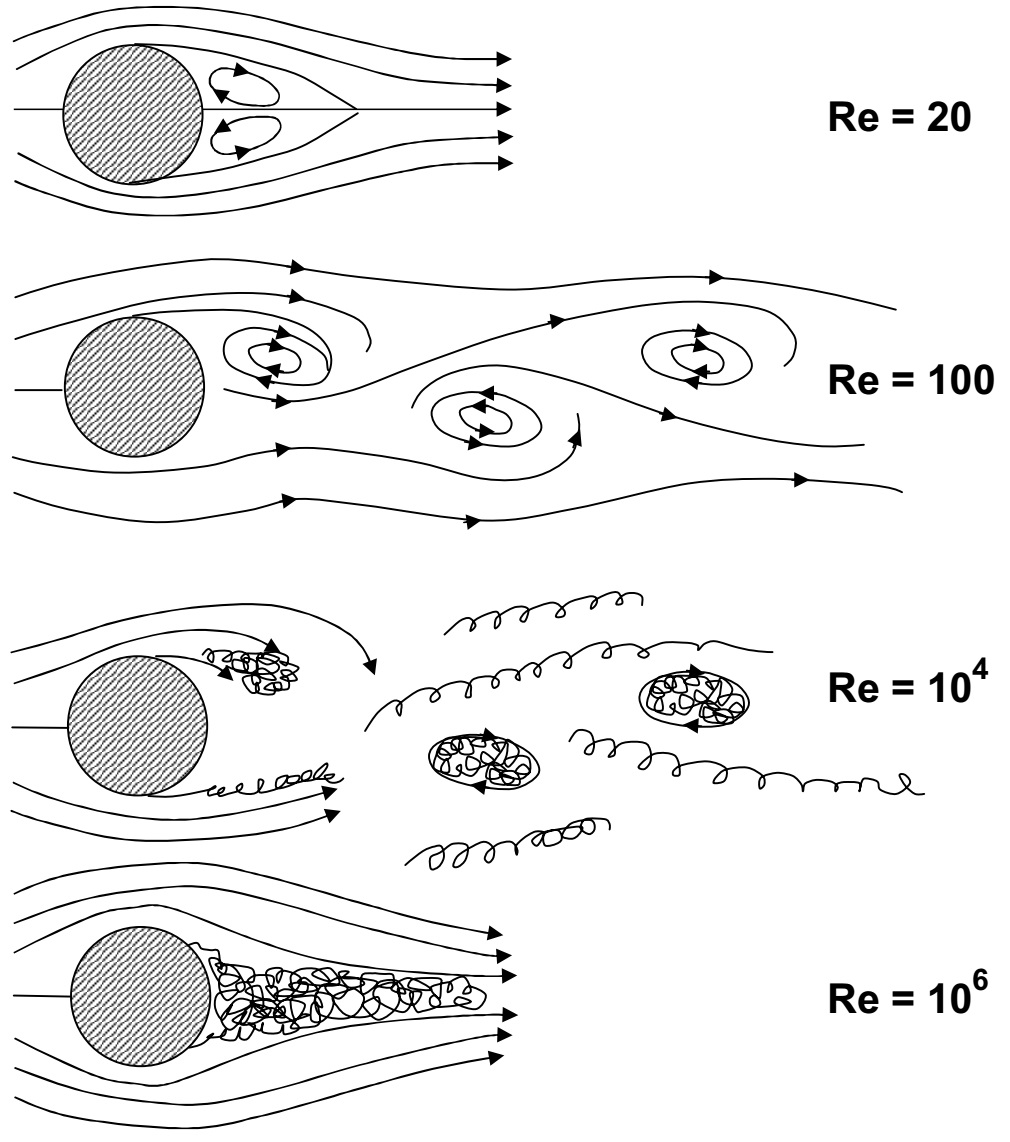
\includegraphics[width=0.5\textwidth]{graphics/theory/laminar-turbulent}
	\caption{Depiction of a classical steady flow for various Reynolds number values. Many phenomena of laminar, semi-turbulent and turbulent flows are visible in depictions. Source:\cite{laminar-turbulence}}
	\label{laminar-turbulent}
\end{figure}

%%%%%%%%%%%%%%%%%%%%%%%%%%%%%%%%%%%%%%%%%%%%%%%%%%%%%%%%%%%%%%%%%%%%%%%%%%%%%%%%%%%%%%%%%%%%%%%%%%%%%%%%%%%%%%%%%%%%%%%%%%%%%%%%%%%%%%%%%%%%%%%%%%%%%%%%%%%%

\section{Hydrodynamics of superfluid}

The macroscopic model is usually called the Hall-Vinen-Bekarevich-Khalatnikov (HVBK) model and provides a generalization of Landau's two-fluid model equations \cite{landau}, including the presence of vortices. We treat the superfluid as a continuum and despite the fact that microscopically the superfluid velocity field is irrotational, we define a macroscopic superfluid vorticity $\vec{\Omega}_s = \nabla \times \vec{v}_s$ accounting for quantized vortices.\\
The downside of this model is its assumption of spatially (not chaotically) organized vortices. The common example is a rotating cylinder \cite{osborne}.\\

The incompressible HVBK equations for normal component $\vec{v}_n (\vec{r}, t)$ and superfluid component $\vec{v}_s (\vec{r}, t)$, respectively, are \cite{barenghi}:

\begin{align}
\frac{\partial\vec{v}_n}{\partial t} + (\vec{v}_n\cdot \nabla)\vec{v}_n =& -\frac{1}{\rho} \nabla P - \frac{\rho_s}{\rho_n} S \nabla T + \frac{\eta}{\rho_n} \nabla^2 \vec{v}_n + \vec{F}_{ns}\,,
\label{motion_normal}\\
\frac{\partial\vec{v}_s}{\partial t} + (\vec{v}_s\cdot \nabla)\vec{v}_s =& -\frac{1}{\rho} \nabla P + S \nabla T + \vec{T} - \frac{\rho_n}{\rho} \vec{F}_{ns}\,,
\hspace{15mm}
\label{motion_super}
\end{align}

where we have defined several quantities:

\begin{align}
\vec{F}_{ns} =
\frac{1}{2} B(T) \vec{\hat{\Omega}} \times [\vec{\hat{\Omega}}_s \times &(\vec{v}_n - \vec{v}_s - \nu_s\nabla \times \vec{\hat{\Omega}}_s)]
\\
+ \frac{1}{2} B^{\prime}(T) \vec{\Omega}_s \times &(\vec{v}_n - \vec{v}_s - \nu_s\nabla \times \vec{\hat{\Omega}}_s)\,,
\end{align}
\begin{equation}
\vec{\hat{\Omega}}_s = \vec{\Omega}_s / \vert \vec{\Omega}_s \vert\,,
\end{equation}
\begin{equation}
\vec{T} = - \frac{\varkappa}{4\pi} \log(b_0 / a_0) \, \vec{\Omega}_s \times (\nabla \times \vec{\hat{\Omega}}_s)
\end{equation}

Here we can identify the quantities as $\vec{F}_{ns}$ (mutual friction force), $\vec{T}$ (vortex tension) and $\eta$ (viscosity parameter). Usually, $b_0$ is the inter-vortex spacing and can be estimated as $b_0 = (2\Omega_s \varkappa)^{-1/2}$ \cite{barenghi}.\\
The HVBK equations have well-defined limiting cases:

\begin{itemize}
	\item $T \rightarrow T_{\lambda}$: In this case $\rho_s \rightarrow 0$ and the normal fluid motion equation (\ref{motion_normal}) becomes the classical Navier-Stokes equation with viscosity term.

	\item $T \rightarrow 0$: In this case $\rho_n \rightarrow 0$ and the superfluid motion equation (\ref{motion_super}) describes a pure (potential) superflow. Additionally, taking the classical limit ($\hbar \rightarrow 0$) would give us the pure Euler equation of inviscid fluid.
\end{itemize}

The HVBK model has been widely used with success to study the transition from the laminar regime to the classical or quantum turbulence, for estimations of critical Reynolds numbers and their temperature dependence.

\newpage

%%%%%%%%%%%%%%%%%%%%%%%%%%%%%%%%%%%%%%%%%%%%%%%%%%%%%%%%%%%%%%%%%%%%%%%%%%%%%%%%%%%%%%%%%%%%%%%%%%%%%%%%%%%%%%%%%%%%%%%%%%%%%%%%%%%%%%%%%%%%%%%%%%%%%%%%%%%%

\section{Dynamical similarity principle}

An important role in the behavior of fluids is taken by the \textit{fluid dimensional numbers}, which are used for scaling of motion equations in fluid mechanics.

The principle of \textit{dynamical similarity} states that two flows of similar geometry have the same dynamical behavior, if they can be characterized by the same set of suitable dimensionless parameters representing transport phenomena. In order to describe Helium-II with correct equations and with the most precision, we have to choose which dimensionless parameters are useful.

\begin{itemize}
	\item \underline{Knudsen number} (Kn): This number helps determine whether statistical mechanics or the continuum mechanics formulation of fluid should be used to model the system. Kn is defined as the ratio of the molecular mean free path $\lambda$ to a representative physical length scale $D$ (container size):
	$\text{Kn} = \lambda / D$.\\
	If the temperature of Helium-II is high enough $T > 1\unit{K}$, there is still sufficient amount of normal component, so the mean free path of thermal excitations is much smaller, comparing it with container scale $\lambda \ll D$. In that case, continuum mechanics could be used as a macroscopic theory for the normal component.

	However, if temperature drops $T \lesssim 0.6 \unit{K}$, mean free path $\lambda$ increases, resulting in $\text{Kn} \sim 1$ and continuum model starts to break down. Here, the system is rather described as a gas of thermal excitations, thus calling it \textit{ballistic regime}.

	\item \underline{Weissenberg number} (Wi): This number relates the typical frequency $\omega$ of occurring fluid perturbations with the characteristic time $\tau$ that describes the relaxation of the fluid towards a thermodynamic equilibrium. The Weissenberg number is then given as a multiplication of this frequency and the relaxation time: $\text{Wi} = \omega \tau$.\\
	Since the relaxation time of Helium-II is relatively small at temperatures $T > 1\unit{K}$, then $\text{Wi} \ll 1$ and Helium-II can be considered as a Newtonian fluid.

	Once again, if temperature drops $T \lesssim 0.6 \unit{K}$, the relaxation time $\tau$ of thermal excitations rises rapidly, resulting in $\text{Wi} \sim 1$, it will cause the fluid to become non-Newtonian.

	\item \underline{Reynolds number} (Re): Let's consider the continuum and Newtonian assumptions ($\text{Kn} \ll 1$ and $\text{Wi} \ll 1$), so the fluid can be described by the raw form of Navier-Stokes (N-S) equation of motion. When we take into account also the incompressibility $\nabla \dotprod \vec{v}_{n,s} = \vec{0}$, the N-S for classical fluid reduces itself to its most simplest form.
	In case of stationary flow ($\partial \vec{v}_{n,s} / \partial t = \vec{0}$), N-S can be rewritten into a dimensionless form \cite{bakalaris}. Following these steps, there arises typical values of velocity $U$ and length scale $L$, at which there is the most significant change in velocity. Reynolds number Re thus can be expressed as a ratio of inertial and dissipative forces as $\text{Re} = U L \rho / \eta$, where $\eta$ is the dynamic viscosity of the flow.\\
	The case of oscillatory flow is described more in the next section.

\end{itemize}

The derivation of the \textit{dynamical similarity} principle can be directly seen from the inspection of the underlying motion equation (\ref{motion_normal}). In the classical fluid dynamics, we use dynamical similarity and dimensionless numbers for expressing various properties of data obtained from experiments.

Alternatively, the dissipative forces are usually described in terms of another  dimensionless number, the \textit{drag coefficient} $C_D$, representing the relation between applied \textit{drag force} $\vec{F}$ and a resulting velocity $\vec{U}$ of a moving object submerged in a fluid:
$$
C_D \!\propto\! U^\alpha, \hspace{1cm}
\text{where}
\left\{
  \begin{array}{l l}
    \alpha=-1 & \quad \text{for slow laminar flows with $\Re \in (0-10)$}\\
    \alpha=0 & \quad \text{for turbulent flows with $\Re \in (10^3-10^5)$}
  \end{array}
\right.\,,
$$

where the laminar case ($C_D \propto 1/U$) represents the viscous skin friction and the turbulent case ($C_D \approx \text{const.}$) represents the pressure drag. It is very common to plot the measured dependence of drag coefficient $C_D$ against the Reynolds number (example in \textbf{Figure \ref{C-Re}}):

\begin{figure}[h]
	\centering
	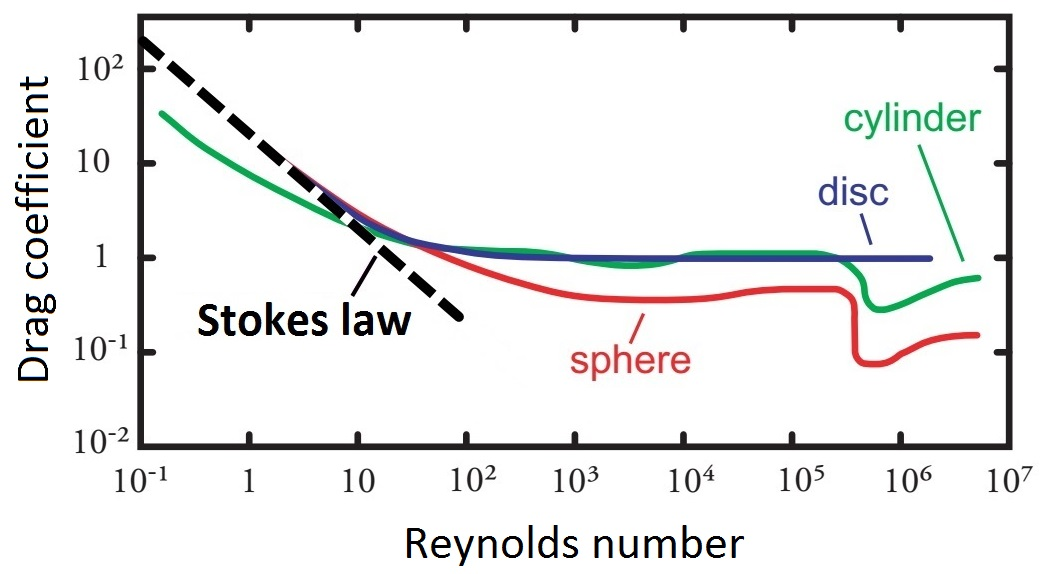
\includegraphics[width=0.7\textwidth]{graphics/theory/C-Re}
	\caption{Drag coefficients $C_D$ of different objects used in a steady flow with changing Reynolds number. \underline{Blue line} - thin disc, \underline{Green line} - cylinder with drag crisis near $\Re \approx 10^6$, \underline{Red line} - sphere with similar drag crisis as with cylinder, \underline{Black dashed line} - laminar fit in the laminar area: $C_D \propto \Re^{-1}$.}
	\label{C-Re}
\end{figure}

Dynamical similarity argument also leads to the existence of critical Reynolds number estimations, at which the transition to turbulent regime occurs in case of classical viscous fluids. Note that since superfluid Helium-II is composed of two fluids, the mentioned applies only to the normal component. The transition of superfluid component to quantum turbulence is described in a more detail in \textbf{Quantum turbulence} section.

%%%%%%%%%%%%%%%%%%%%%%%%%%%%%%%%%%%%%%%%%%%%%%%%%%%%%%%%%%%%%%%%%%%%%%%%%%%%%%%%%%%%%%%%%%%%%%%%%%%%%%%%%%%%%%%%%%%%%%%%%%%%%%%%%%%%%%%%%%%%%%%%%%%%%%%%%%%%

\section{Oscillatory flows}

If a given body is oscillating in a classical viscous fluid, described by ordinary Navier-Stokes equation, there appears another characteristic length scale, at which the oscillations attenuate, identified \cite{landau} \cite{bakalaris} as the \textit{viscous penetration depth}:

\begin{equation}
\delta(\omega) = \sqrt{\frac{2\eta}{\rho\omega}}\,,
\label{penetration}
\end{equation}

where $\omega$ is the angular frequency of oscillations.

In order to calculate the Reynolds numbers correctly, we have to recognize the correct characteristic length scale (whether it should be the dimension $D$ of the oscillating body or its penetration depth $\delta(\omega)$).\\
For this purpose, we define another dimensionless quantity, the \underline{Stokes number} $\beta$, as the ratio of time-dependent term $\partial \vec{v} / \partial t$ from N-S equation (\ref{motion_normal}) to the viscous term $\nabla^2 \vec{v}$.
We calculate the Stokes number \cite{stokes} as $\beta = \omega \rho D^2 / (\pi \eta)$, which can be reduced using (\ref{penetration}) to $\beta = D^2 / (\pi \delta^2)$.\\
According to this definition, we call the flow characteristics as the \textit{high-frequency limit}, when the Stokes values are $\beta \gg 1$, so the penetration depth $\delta \ll D$. Consequently, the right choice for the characteristic length depends on this limitation.

%%%%%%%%%%%%%%%%%%%%%%%%%%%%%%%%%%%%%%%%%%%%%%%%%%%%%%%%%%%%%%%%%%%%%%%%%

\subsection*{Classical hydrodynamics}

To describe fully an oscillatory flow for the classical viscous fluid, the governing Navier-Stokes equation may be expressed in terms of dimensionless velocity $U$, time $T$ and positions $L$. The independent time scale is given by the angular frequency of oscillations $\omega$. Candidates for characteristic length scale $L$ may lead to the body size $D$, viscous penetration depth $\delta(\omega)$ or eventually to the surface roughness.

To reach the high-frequency limit, the condition directly from \ref{penetration} for the oscillation frequency: $\omega \gg 2\eta / (\rho D^2)$ has to be fulfilled. Depending on body geometry, one can reach $\delta(\omega) \ll D$ and say that fluid oscillates in high-Stokes regime $\beta \gg 1$.

Also, when the surface roughness is sufficiently negligible, the laminar-turbulent transition may be finally expressed using a single dimensionless parameter: an \textit{oscillatory Reynolds number} $\Re_{\delta} = U \delta \rho / \eta$.

%%%%%%%%%%%%%%%%%%%%%%%%%%%%%%%%%%%%%%%%%%%%%%%%%%%%%%%%%%%%%%%%%%%%%%%%%%

\subsection*{Superfluid Helium-II}

Assuming two independent velocity fields $\vec{v}_n (\vec{r}, t)$, $\vec{v}_s (\vec{r}, t)$ as the normal and superfluid components in superfluid Helium-II, the above thoughts are applicable for the oscillatory viscous flow of the normal component. We therefore define the high frequency limit for normal component as:

\begin{equation}
\delta_n = \sqrt{\frac{2\eta}{\rho_n\omega}}\,,
\hspace{1cm}
\text{Dn} = \frac{U \delta_n \rho_n}{\eta}
\label{donnelly}\,,
\end{equation}

We will call the oscillatory Reynolds number for normal component in superfluid Helium-II as a \textit{Donnelly number} with the abbreviation Dn, after Russell J. Donnelly, who as first came with this (\ref{donnelly}) idea.

At low velocities, below any critical thresholds for creating either classical or quantum turbulence, the flow of the superfluid component is expected to be purely potential and the normal component exhibiting laminar viscous flow.

Moreover, if the typical body curvature is of order $1/D$, the surface may be described as if consisting of many planar elements. In this case it is shown \cite{universal_scaling} that we can write for the average dissipated energy:

\begin{equation}
\langle \dot{E} \rangle =
\frac{1}{2} \alpha \xi U_0^2 S_{eff} \sqrt{\frac{\eta \rho_n \omega}{2}}\,,
\label{energy_loss}
\end{equation}

where $U_0$ is the velocity amplitude, $S_{eff}$ the effective surface, $\alpha$ the \textit{flow enhancement constant} (depending on object geometry) and $\xi$ the integral of velocity profile along the resonator. The total energy of an oscillator is given as $E = \xi m U_0^2 / 2$ and moreover, we define a fluidic quality factor $Q_f$ of an oscillator for a single oscillation as:

\begin{equation}
1 / Q_f = \frac{\langle \dot{E} \rangle}{\omega E} = \frac{\alpha \rho_n S_{eff} \delta_n}{2m}
\label{quality}
\end{equation}

From (\ref{energy_loss}), one can also derive the peak dissipative force (during a period of oscillation) and the dimensionless drag coefficient related to the normal component:

\begin{equation}
F_0 = \frac{2 \omega \langle \dot{E} \rangle}{U_0}
= \alpha \xi \omega S_{eff} U_0 \sqrt{\frac{\eta \rho_n \omega}{2}}
\hspace{5mm}
\rightarrow
\hspace{5mm}
C_D^{\,n} = \frac{2 F}{A \rho_n U_0^2} = \frac{2 S_{eff}}{A U_0} \sqrt{\frac{\eta \omega}{\rho_n}}\,,
\label{drag_normal}
\end{equation}

where $A$ is the cross-section of the body perpendicular to flow. According to dynamical similarity principle, the drag coefficient (\ref{drag_normal}) can be expressed as a function of the dimensionless Donnelly number (\ref{donnelly}):

\begin{equation}
C_D^{\,n} = \Phi / \text{Dn}\,,
\end{equation}

where number $\Phi$ is determined by the oscillating body geometry. Clearly, the laminar behavior of the normal component is fully described by the classical hydrodynamic laws, whereas in turbulent case, we expect a constant value for $C_D^{\,n}$ as long, as only normal component contributes to the drag force (no quantized vortices present).

%%%%%%%%%%%%%%%%%%%%%%%%%%%%%%%%%%%%%%%%%%%%%%%%%%%%%%%%%%%%%%%%%%%%%%%%%%%%%%%%%%%%%%%%%%%%%%%%%%%%%%%%%%%%%%%%%%%%%%%%%%%%%%%%%%%%%%%%%%%%%%%%%%%%%%%%%%%%%%%%%%%%%%%%%%%%

\section{Quantum turbulence}

Turbulence of superfluid component can be viewed as a tangle of vortex lines, causing the drag due to their motion. Quantized vortices can be nucleated either \textit{intrinsically}, by exceeding a critical velocity of order $10 \unit{m/s}$ ,or \textit{extrinsically}, by stretching and reconnecting of vortex loops. The initial vortices in the extrinsic case are the \textit{remnant vortices}, which always exist in macroscopic samples of Helium-II. This type of vortex nucleation is also driven by the excess of critical velocity, which is observed to be in order $\sim\unit{cm/s}$ and heavily depends on the motion characteristics of an object.

Let's say the superfluid component becomes turbulent at some critical velocity $U_C$. In such case we expect an increase in drag coefficient $C_D$ much above the possible dependence caused by turbulence of normal component. The process of self-reconecting remnant vortices due to body oscillatory motion was well studied \cite{universal_scaling} and the related critical velocity is expected to scale as $U_C \propto \sqrt{\varkappa \omega}$, where $\varkappa$ is the circulation quantum and $\omega$ is the oscillation frequency. Hence, it is convenient to define a dimensionless velocity $\hat{U}$ with related drag coefficient $C_D^{\,s}$ as:

\begin{equation}
\hat{U} = U_0 / \sqrt{\varkappa \omega}
\hspace{5mm}
\rightarrow
\hspace{5mm}
C_D^{\,s} = \frac{2 F_0}{A \rho_s U_0^2} = \frac{2 F_0}{A \rho_s \varkappa \omega \hat{U}^2}
\label{drag_super}
\end{equation}

If we consider the superfluid component (a dense tangle of quantized vortices) to be already turbulent with velocities sufficiently above critical values, we expect both normal and superfluid components to be coupled due to the mutual friction. Normal component could be then easily triggered to become turbulent as well, so both components contribute to the pressure drag. In this case, the drag coefficient must be calculated classically as $C_D = 2F_0 / (A\rho U_0^2)$. where $\rho$ is the total density of Helium-II.

\newpage

\subsection*{Ultra-low temperature regime}

In classical fluids, when the mean free path $\lambda$ of particles becomes comparable to a length scale $D$ of the system ($\text{Kn} \sim 1$), the continuum model of the fluid starts to break down and the system can no longer be described by the Navier-Stokes equations. Similar arguments go when time period of oscillatory flow $1/\omega$ becomes comparable with the relaxation time $\tau$ of the fluid towards thermodynamic equilibrium ($\text{Wi} \sim 1$).\\
Considering this, the system is no longer be described as a continuum, but rather as a gas of thermal quasiparticles propagating ballistically through a physical vacuum. Therefore, we call this state as the \textit{ballistic regime}.

In practice, the ballistic regime is usually reached by cooling fluid down to ultra-low temperatures $T < 0.6\unit{K}$ where the normal component accounts for less than $1\%$ of the total density. However, the Knudsen number increases unusually faster than the Weissenberg number, as plotted in \textbf{Figure \ref{Kn-Wi}}.

\begin{figure}[h]
	\centering
	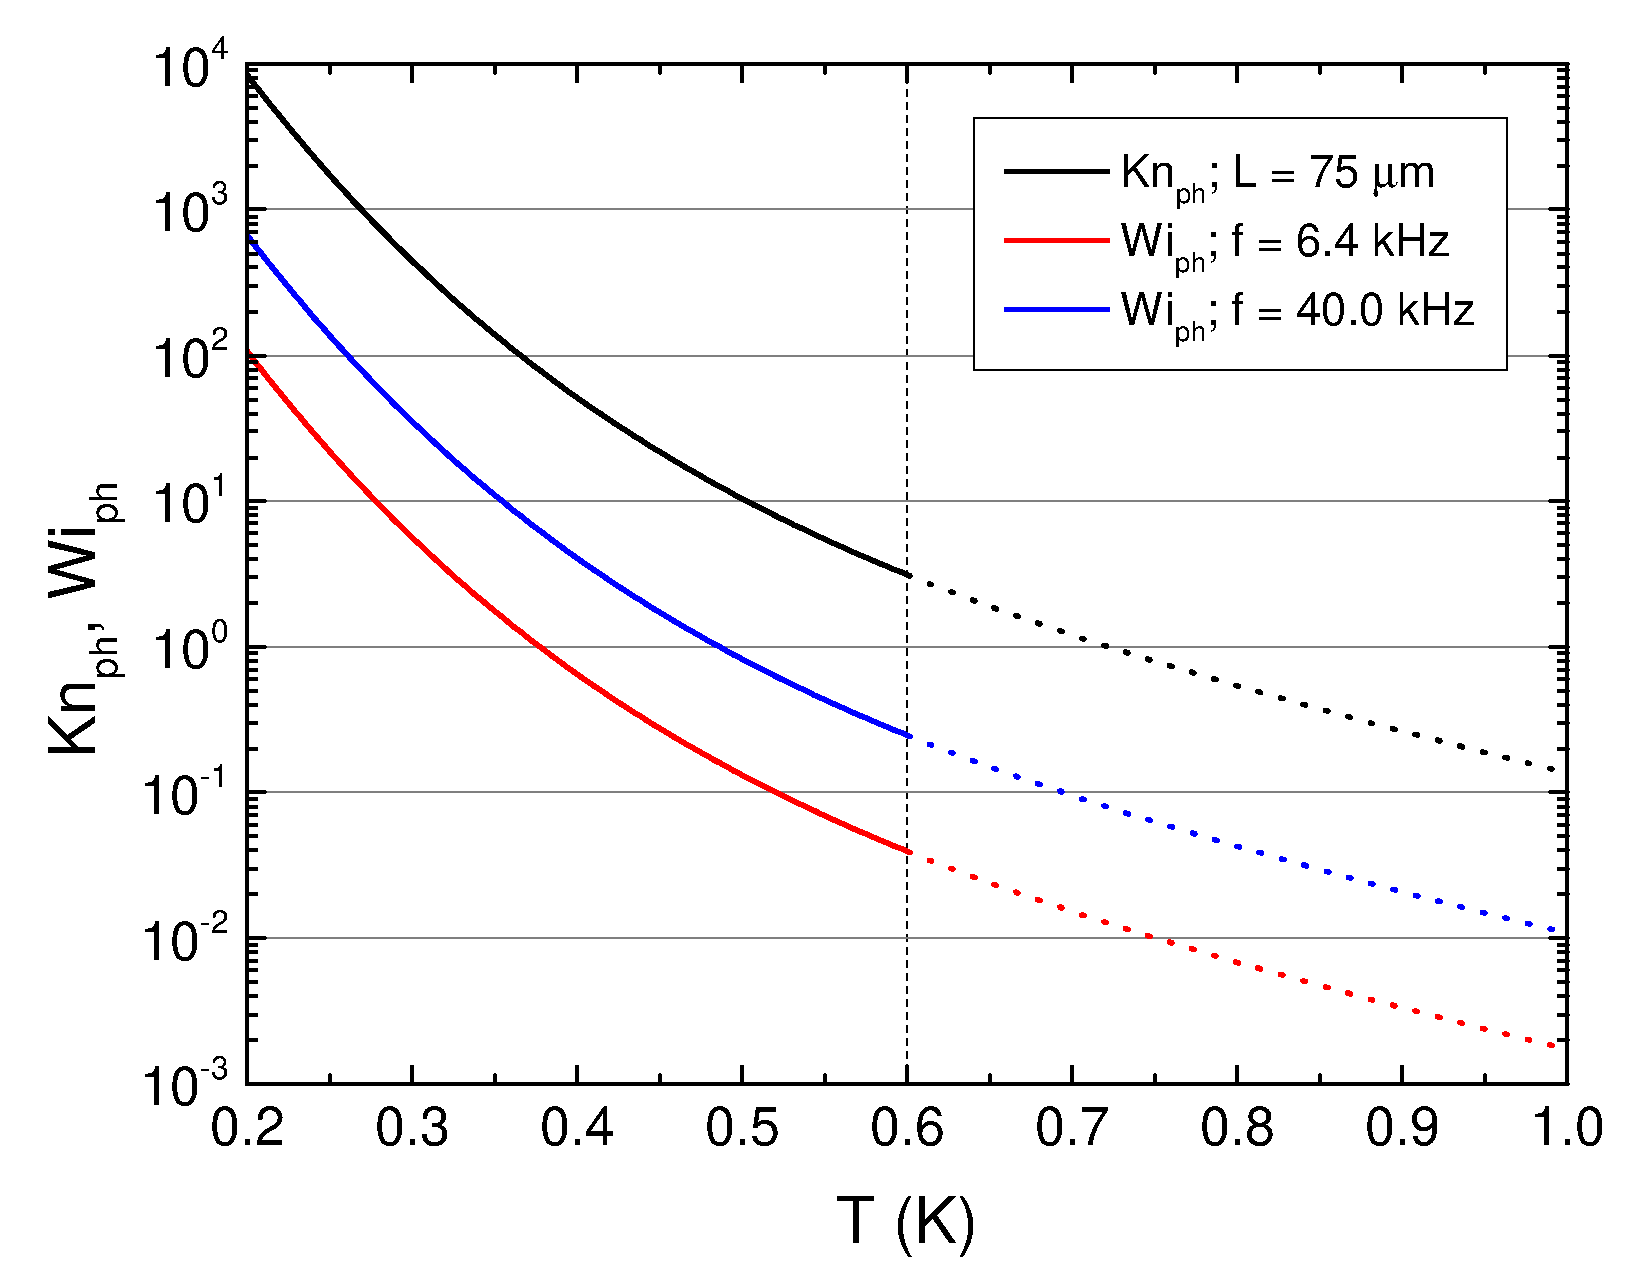
\includegraphics[width=0.7\textwidth]{graphics/theory/ballistic}
	\caption{Plot of phonon Knudsen number and Weissenberg numbers against a range of temperatures for the fundamental and overtone modes of the tuning fork. The dashed line separates the interval $T < 0.6\unit{K}$, where the description of Helium-II as a gas of phonons is valid. Source:\cite{universal_scaling}}
	\label{Kn-Wi}
\end{figure}

\newpage

\section{Universal scaling}

A study was conducted in order to solve the Stokes' second problem with an oscillating plane in viscous fluid, using the Boltzmann kinetic equation. This solution was used to derive a universality relation valid in the high-frequency limit and at low velocities, thus with no turbulence present (neither classical nor quantum). This relation holds across both Newtonian and non-Newtonian regimes of the fluid.

A newly introduced scaling function $f(\text{Wi})$, derived by the authors in \cite{universal_scaling}, relates the quality factor of an oscillator (\ref{quality}) with the geometric and hydrodynamic parameters:

\begin{equation}
1 / Q_f = \frac{\alpha S_{eff}}{m} \sqrt{\frac{\eta \rho_n}{2\omega}} f(\text{Wi})\,,
\label{scaling_function}
\end{equation}

where the scaling function $f(\text{Wi})$ is the added term and is defined as:

\begin{equation}
f(\text{Wi}) = \frac{(1 + \text{Wi}) \cos{\phi} - (1 - \text{Wi}) \cos{\phi}}{(1+\text{Wi})^{3/4}}
\label{f-Wi}
\end{equation}
\begin{equation}
\phi = \frac{\tan{\text{Wi}^{-1}}}{2}
\end{equation}

In addition to the authors' original suggestion, we have explicitly included the flow enhancement factor $\alpha$, which is necessary to recover the analytical solutions for drag on a sphere or a cylinder.

In hydrodynamical regime, when there is enough normal component present $T > 1\unit{K}$, the limit $\text{Wi} \ll 1$ clearly shows the constant behavior of scaling function $f(\text{Wi}) \rightarrow 1$. However, when Wi reaches the critical value $\text{Wi} \sim 1$, the scaling function increases and in an extreme non-Newtonian case when $\text{Wi} \ll 1$, the scaling function converges to the relation $f(\text{Wi}) \propto \text{Wi}^{-1/2}$.\\
In the hydrodynamical regime, the relaxation time of the normal component is closely related with the viscosity, which leads to the estimation of Weissenberg number: $\text{Wi} \approx \eta \omega / (\rho_n c_2^2)$, where $c_2$ is the velocity of second sound wave.

Finally, this allows us to use the scaling relation both for the hydrodynamical regime ($T > 1\unit{K}$) and the phonon gas ($T \lesssim 0.6\unit{K}$), so the fluidic quality factor can be rewritten:

\begin{equation}
1 / Q_f = \frac{\alpha S_{eff} \rho_x c_2}{m\omega} \sqrt{\text{Wi}/2} f(\text{Wi})\,,
\end{equation}

where $\rho_x$ means either normal component $\rho_n$ or phonon density $\rho_{ph}$.

In \textbf{Results} chapter we use this form of universality scaling for comparison against experimental data collected in both temperature ranges $T > 1\unit{K}$ and $T < 0.6\unit{K}$ .

\subsection*{Multiple critical velocities}

Here is briefly commented the transition to quantum turbulence regime observed at very low temperatures ($T \ll 1\unit{K}$). A couple of experimental studies in milliKelvin temperatures reported \cite{crit-velocity} the existence of more critical velocities related with superfluid component flow within single experiment:

\begin{itemize}
	\item \underline{First critical velocity} is related to the formation of pinned vortex loops at the surface of oscillating body - possibly forming a thin layer with different hydrodynamic behavior which increases the effective mass of the oscillating object. Such critical velocity is hard to observe at higher than ultra-low temperatures.

	\item \underline{Second critical velocity} is a consequence of vortex rings escaping from the oscillator body into the superfluid bulk and eventually forming a vortex tangle. Here the sudden raise of drag is observed, usually with hysteresis effect.

	\item \underline{Third critical velocity} is the highest critical velocity of order $\sim\unit{m/s}$ which can be observed. The origin of this velocity is linked to the development of larger quantized vortex structures, which in larger scale start to mimic the classical turbulence. Due to the high value of this critical velocity, it is not likely reachable within experiments reported in this Thesis.
\end{itemize}

\subsection*{Additional dissipation mechanisms}

In addition to expected viscous drag and a drag caused by the created vortex tangle, the losses in energy may be caused also due to the sound emissions through the surrounding fluid.

In this Thesis, such sound emissions can be completely neglected, based on previous studies \cite{emission} \cite{fork-exp} of acoustic emissions by oscillating object in Helium-II. Perhaps a very small contribution could occur in the first overtone mode of oscillated tuning fork (explained in more detail in \textbf{Experimental approach})

% When both velocities of Helium-II are high enough, we expect the turbulent regime on both sides to be coupled due to mutual friction and contributing to the drag. In such situation, we are forced to use classical hydrodynamic metrics: drag coefficient $C_D = 2F / (A\rho U^2)$ and Donnelly number $D = U \delta / \nu$. Recent researches also hint that both classical turbulent and quantum turbulent regimes can exist separately with low interaction.
%
% Note that all presented approaches are only approximate, since they are neglecting flows near the oscillating body, evaporation processes, sound emissions and other corner-case effects.

% \section{Second sound}
%
% Ordinary sound (the wave of density $\rho$ and pressure $P$) in Helium-II is called \textit{first sound}. In such process, temperature $T$ and entropy $S$ is conserved and $\vec{v}_n$ and $\vec{v}_s$ oscillate in phase with each other ($\vec{v}_n(t) \approx \vec{v}_s(t)$). On the contrary, by combination of two-fluid motion and continuity equations, one obtains the wave equation also for the temperature $T$ and entropy $S$. In such case the velocities obey an anti-phase oscillation ($\rho_n(t) \vec{v}_n(t) \approx - \rho_s(t) \vec{v}_s(t)$) and remains $\rho$ and $P$ constant.
%
% \begin{figure}[h]
% 	\centering
% 	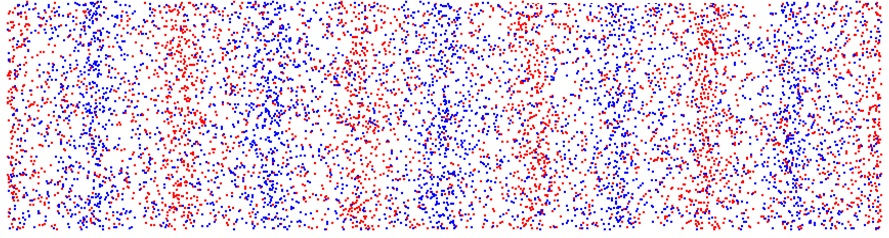
\includegraphics[width=0.99\textwidth]{graphics/theory/ss_1}
% 	\caption{here will come more proper picture}
% 	\label{ss_1}
% \end{figure}
%
% \begin{figure}[h]
% 	\centering
% 	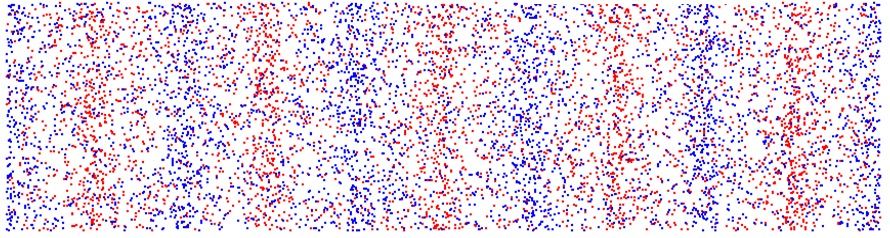
\includegraphics[width=0.99\textwidth]{graphics/theory/ss_2}
% 	\caption{here will come more proper picture}
% 	\label{ss_2}
% \end{figure}
%
% In early Vinen's observations, the exponentially damped velocity of second sound wave, propagating through two-fluid medium, was derived from motion equations:
%
% \begin{equation}
% \vec{v}_{\ind{ns}} \propto e^{-\alpha \vert \vec{r} \vert} \vec{\hat{e}}_{\vec{r}}(\vec{k},\vec{r},\omega,t)\,,
% \end{equation}
%
% where $\alpha$ is the attenuation coefficient. When considering homogeneous chaotic distribution of vortex tangle, one can also derive the formula for the attenuation factor:
%
% \begin{equation}
% \alpha = \frac{B\kappa L}{6 \vert \vec{c}_2\vert}
% \label{alpha_mean}\,,
% \end{equation}
%
% where $B$ is the first mutual friction parameter and $\vec{c_2}$ is the initial second sound velocity. This velocity was experimentally examined and there was found a plateau near the value $20 \unit{m/s}$, which is desirable during experiments (stability against small temperature changes):
%
% \begin{figure}[h]
% 	\centering
% 	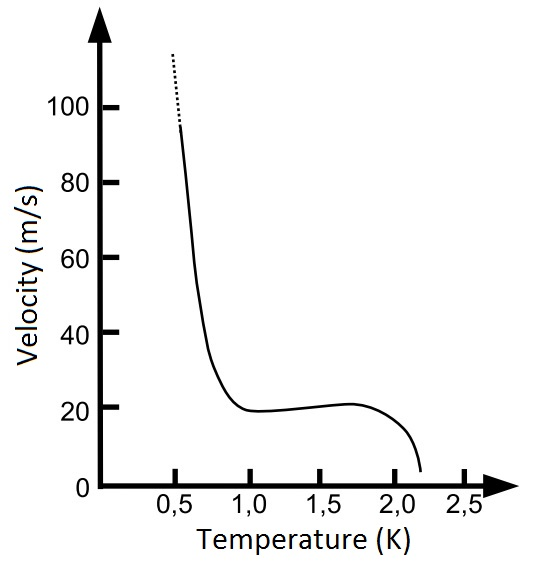
\includegraphics[width=0.4\textwidth]{graphics/theory/ss_velocity}
% 	\caption{velocity of the second sound with temperature}
% 	\label{ss_velocity}
% \end{figure}
%
% In this work, the phenomenon of second sound attenuation is used for detection of quantized vortices, which naturally appear within Helium-II. There is written much more about the method itself within the Experimental Approach part.

\newpage
